\section{Graphical Gradients or ``Spread"}
\label{section:spread}

\subsection{Graphical Spread Theory}
\label{subsection:spreadtheory}

Another way we can use to understand the mixing direction and how well surfaces of interest align with it is to graphically look at the spread of thermodynamic variables on said surfaces.  In order to see whether a surface aligns well with the mixing direction we can project $\theta$ and $S$ onto the surface and then analyse the ``spread" of these properties. As before in section \ref{subsection:gradienttheorymathematicaltheory}, the better a surface aligns with the mixing direction, the smaller the ``spread" should be \citet{McDougall1987}. 

An example of this is given in figure 9 in \citet{McDougall1987}. Below in figure \ref{fig:theory_mcdougall_theta_spread} we can see $\theta$ projected onto four different surfaces. It can be seen that the ``spread" is smallest in figure \ref{fig:theory_mcdougall_theta_spread}(d) on the $\sigma_2 = 36.84$ surface. The largest ``spread" is on $\sigma_0 = 27.73$, while the neutral surface has a smaller ``spread" than $\sigma_0 = 27.73$ but larger than $\sigma_2 = 36.84$. This suggests that, contrary to what \citet{McDougall1987} claimed, $\sigma_2 = 36.84$ is actually better aligned with the mixing direction in this case. 

\begin{figure}[htbp]
    \centering
    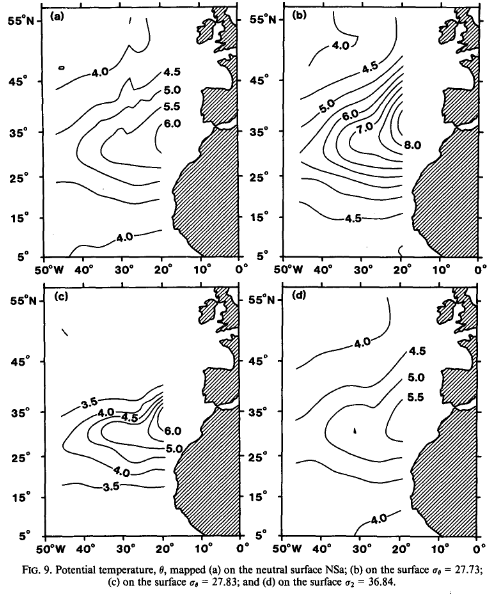
\includegraphics{mcdougall_fig_9}
    \caption{Potential temperature, $\theta$, mapped onto (a) neutral surface ``Nsa", referred to as $\gamma_n = 27.87$ in this paper (b) $\sigma_0 = 27.73$ (c) $\sigma_0 = 27.83$ and (d) $\sigma_2 = 36.84$ \citep{McDougall1987}}
    \label{fig:theory_mcdougall_theta_spread}
\end{figure}

While this provides a more intuitive way of understanding a surface's alignment with the mixing direction, sometimes the results can be less clear than the mathematical formulation. As such, these graphs should be used to confirm mathematical theory or expectations rather as standalone proof. 



